% \documentclass{article}
\documentclass[margin=20pt]{standalone}

\usepackage{cjhebrew}
\usepackage{tikz}
\usetikzlibrary[calc]
\usetikzlibrary[decorations.text]

\begin{document}
  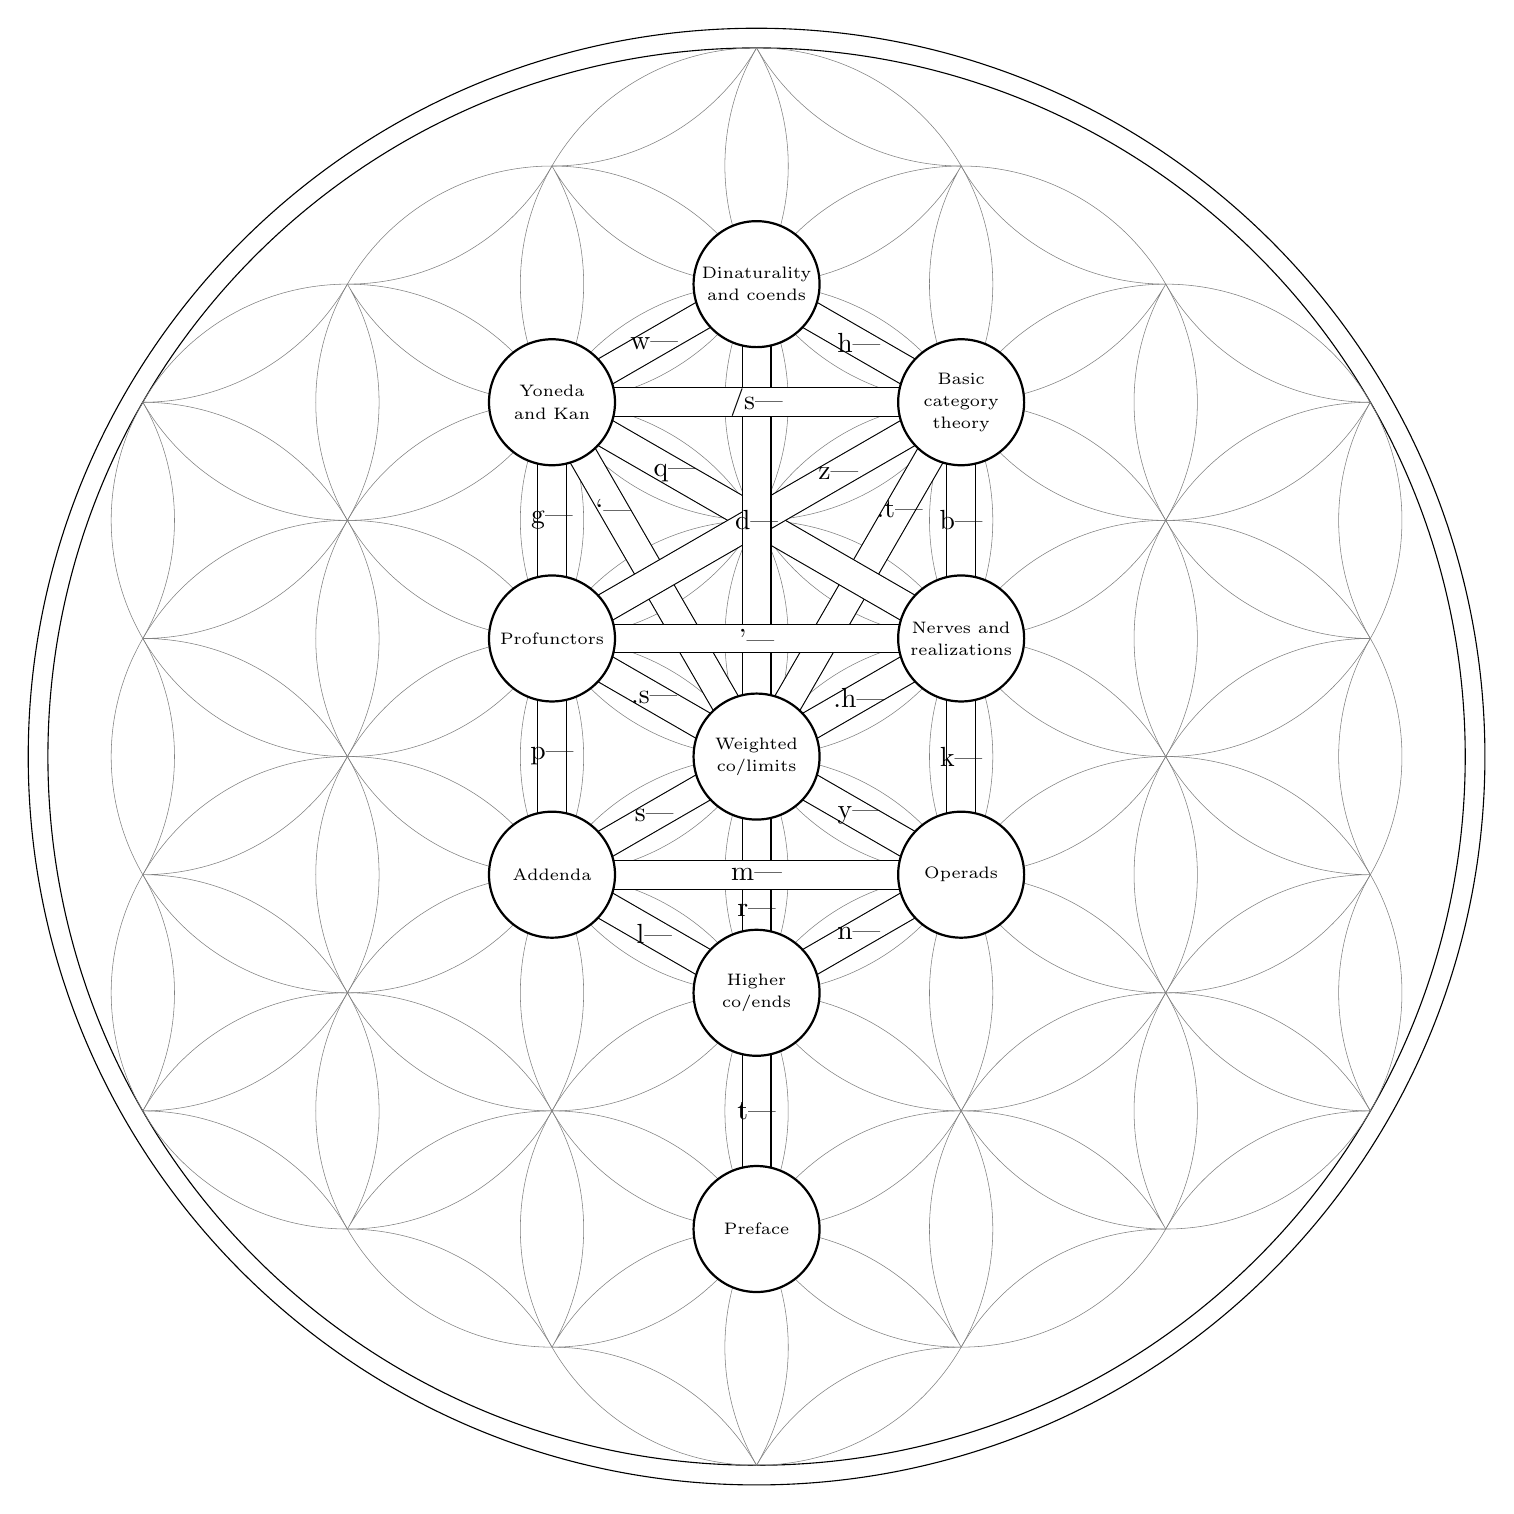
\begin{tikzpicture}[
      x={ 3cm*sin(60)},
      y={-3cm*cos(60)},
      sephirot/.style={
        draw,
        fill=white,
        line width=.8pt,
        shape=circle,
        inner sep=0sp,
        minimum size=1.6cm,
        text width=1.4cm,
        font=\fontsize{6pt}{8pt}\selectfont,
        align=center,
      },
      sibihil/.style={
        line width=.4pt,
        double distance=10pt,
      },
      mosaic/.style={
        line width=.2pt,
        gray
      },
      frame/.style={
        line width=.4pt,
      }
    ]
    % Reference points
    \coordinate (S0) at ( 0,0);
    \coordinate (S1) at (-1,1);
    \coordinate (S2) at (+1,1);
    \coordinate (S3) at (-1,3);
    \coordinate (S4) at (+1,3);
    \coordinate (S5) at ( 0,4);
    \coordinate (S6) at (-1,5);
    \coordinate (S7) at (+1,5);
    \coordinate (S8) at ( 0,6);
    \coordinate (S9) at ( 0,8);
    % Frame
    \draw[frame] (0,4) circle (3*3cm);
    \draw[frame] (0,4) circle (3*3cm+.25cm);
    % Hexagonal pattern
    \draw[mosaic] (-2,2) circle (3cm);
    \draw[mosaic] (-2,4) circle (3cm);
    \draw[mosaic] (-2,6) circle (3cm);
    \draw[mosaic] (-1,1) circle (3cm);
    \draw[mosaic] (-1,3) circle (3cm);
    \draw[mosaic] (-1,5) circle (3cm);
    \draw[mosaic] (-1,7) circle (3cm);
    \draw[mosaic] ( 0,0) circle (3cm);
    \draw[mosaic] ( 0,2) circle (3cm);
    \draw[mosaic] ( 0,4) circle (3cm);
    \draw[mosaic] ( 0,6) circle (3cm);
    \draw[mosaic] ( 0,8) circle (3cm);
    \draw[mosaic] (+1,1) circle (3cm);
    \draw[mosaic] (+1,3) circle (3cm);
    \draw[mosaic] (+1,5) circle (3cm);
    \draw[mosaic] (+1,7) circle (3cm);
    \draw[mosaic] (+2,2) circle (3cm);
    \draw[mosaic] (+2,4) circle (3cm);
    \draw[mosaic] (+2,6) circle (3cm);
    \draw[mosaic] (0,-2)
      arc (-150:-90:3cm)
      arc (-150:-90:3cm)
      arc (-150:-90:3cm)
      arc (150:210:3cm)
      arc (150:210:3cm)
      arc (150:210:3cm)
      arc (90:150:3cm)
      arc (90:150:3cm)
      arc (90:150:3cm)
      arc (30:90:3cm)
      arc (30:90:3cm)
      arc (30:90:3cm)
      arc (-30:30:3cm)
      arc (-30:30:3cm)
      arc (-30:30:3cm)
      arc (-90:-30:3cm)
      arc (-90:-30:3cm)
      arc (-90:-30:3cm)
    ;
    \draw [mosaic] (0,-2)
      arc (-210:-30:3cm)
      arc (-210:-90:3cm)
      arc (-270:-90:3cm)
      arc ( 30:210:3cm)
      arc ( 30:150:3cm)
      arc (-30:150:3cm)
      arc (-90:90:3cm)
      arc (-90:30:3cm)
      arc (-150:30:3cm)
    ;
    \draw [mosaic] (0,10)
      arc (-30:150:3cm)
      arc (-30:90:3cm)
      arc (-90:90:3cm)
      arc (-150:30:3cm)
      arc (-150:-30:3cm)
      arc (-210:-30:3cm)
      arc (-270:-90:3cm)
      arc (-270:-150:3cm)
      arc (30:210:3cm)
    ;
    % Outer edges
    \draw[sibihil] (S9) -- (S8) node[midway] {\textcjheb{t|}};
    \draw[sibihil] (S8) -- (S7) node[midway] {\textcjheb{n|}};
    \draw[sibihil] (S7) -- (S4) node[midway] {\textcjheb{k|}};
    \draw[sibihil] (S4) -- (S2) node[midway] {\textcjheb{b|}};
    \draw[sibihil] (S2) -- (S0) node[midway] {\textcjheb{h|}};
    \draw[sibihil] (S0) -- (S1) node[midway] {\textcjheb{w|}};
    \draw[sibihil] (S1) -- (S3) node[midway] {\textcjheb{g|}};
    \draw[sibihil] (S3) -- (S6) node[midway] {\textcjheb{p|}};
    \draw[sibihil] (S6) -- (S8) node[midway] {\textcjheb{l|}};
    % Inner edges
    \draw[sibihil] (S5) -- (S8) node[pos=.65] {\textcjheb{r|}};
    \draw[sibihil] (S5) -- (S7) node[midway] {\textcjheb{y|}};
    \draw[sibihil] (S5) -- (S4) node[midway] {\textcjheb{.h|}};
    \draw[sibihil] (S5) -- (S2) node[pos=.7] {\textcjheb{.t|}};
    \draw[sibihil] (S5) -- (S1) node[pos=.7] {\textcjheb{`|}};
    \draw[sibihil] (S5) -- (S3) node[midway] {\textcjheb{.s|}};
    \draw[sibihil] (S5) -- (S6) node[midway] {\textcjheb{s|}};
    \draw[sibihil] (S1) -- (S4) node[pos=.3] {\textcjheb{q|}};
    \draw[sibihil] (S2) -- (S3) node[pos=.3] {\textcjheb{z|}};
    \draw[sibihil] (S5) -- (S0) node[midway] {\textcjheb{d|}};
    \draw[sibihil] (S1) -- (S2) node[midway] {\textcjheb{/s|}};
    \draw[sibihil] (S3) -- (S4) node[midway] {\textcjheb{'|}};
    \draw[sibihil] (S6) -- (S7) node[midway] {\textcjheb{m|}};
    % Nodes
    \node[sephirot] at (S0) {Dinaturality and coends};
    \node[sephirot] at (S1) {Yoneda and Kan};
    \node[sephirot] at (S2) {Basic category theory};
    \node[sephirot] at (S3) {Profunctors};
    \node[sephirot] at (S4) {Nerves and realizations};
    \node[sephirot] at (S5) {Weighted co/limits};
    \node[sephirot] at (S6) {Addenda};
    \node[sephirot] at (S7) {Operads};
    \node[sephirot] at (S8) {Higher co/ends};
    \node[sephirot] at (S9) {Preface};
  \end{tikzpicture}
\end{document}
